
% BEGIN COMPLETE NATIVE SECULAR AND FRAME PROOFS

\clearpage\begingroup
\part*{The original odd receiving divisor and one-moment recovery}
\newtheorem{sfrepairtheorem}{Theorem}
\newtheorem{sfrepairproposition}[sfrepairtheorem]{Proposition}
\newcommand{\sfrepairC}{\mathbb C}
\newcommand{\sfrepairdd}{\mathfrak D_{\rm odd}}
\newcommand{\sfrepairrem}{\operatorname{rem}}
\newcommand{\sfrepairdiag}{\operatorname{diag}}


\section{The original maps and the scope of this calculation}
The original four-coordinate Fable receiving map has eight marked states
over a squarefree quartic. This note proves that its particular odd
evaluation frame can become singular while all eight states remain
regular, and calculates a minimal observation that recovers the lost
direction. The original source's arithmetic-quartet invertibility
remains valid: its exact pullback is proved below, with the original
leading coefficient retained. The general target used to exhibit the
new divisor is not asserted to be a quartet of zeta zeros.

The received formulas and proposed repair are attributed to the
user-supplied web-session calculation \cite{sfrepair:Incoming}; the original
marked-state construction is \cite[SE1--14, GF20--21]{sfrepair:Fable}.
The classical interpolation used in the null-vector calculation is
Lagrange interpolation, in the original equation sources of
N.~M.~Temme \cite{sfrepair:Temme}. Every polynomial identity needed here is
also proved below; the accompanying exact rational script verifies
their coefficient equalities without substituting numerical roots.

Let $u=(A,B,C,D)\in\sfrepairC^4$, with $A\ne0$, and
\begin{equation}
 h(r)=Ar^4+r^3+Br^2+Cr+D,\quad d(r)=h'(r).
 \tag{OF1}
\end{equation}
Assume $h$ has four distinct roots in a fixed order $r_1,\ldots,r_4$.
Choose and retain $\xi_j^2d(r_j)=1$. The eight original columns are
$p_j^\pm=e_j\pm o_j$, where
\begin{equation}
 e_j=\begin{pmatrix}0\\-r_j\\3i d_j\\
 (B-17r_j+Ar_j^2)d_j-2Ad_j^2\end{pmatrix},\qquad
 o_j=\xi_j\begin{pmatrix}1\\-id_j\\Ad_j^2+2r_jd_j\\
 i(7r_j^2d_j-13d_j^2)\end{pmatrix},\quad d_j=d(r_j).
 \tag{OF2}
\end{equation}
For $E=[e_j]$, $O=[o_j]$, and literal branch coefficients $c_j^\pm$,
\begin{equation}
 \alpha_j=c_j^++c_j^-,\quad\beta_j=c_j^+-c_j^-,\quad
 \sum_j(c_j^+p_j^++c_j^-p_j^-)=E\alpha+O\beta,\quad
 c_j^\pm=(\alpha_j\pm\beta_j)/2.\tag{OF3}
\end{equation}
These formulas specify all domains and inverses between the marked
eight-dimensional coefficient space and its even/odd coordinates.
An original invertible linear conductor $L:\sfrepairC^4\to\sfrepairC^4$ composes
as $LO$ and satisfies $\det(LO)=\det L\det O$. Thus the receiving
divisor computed here is carried through that conductor unchanged.

\section{The complete divisor and its arithmetic pullback}
\begin{sfrepairtheorem}
Put
\begin{align}
 \sfrepairdd={}&20(3C-B^2)+A(87B^3-282BC-51D)\notag\\
 &+A^2(-28B^4+22B^2C+431C^2+204BD)\notag\\
 &+A^3(224B^2D-168BC^2-856CD)-448A^4D^2.
 \tag{OF4}
\end{align}
Then, for the retained branch ordering and signs,
\begin{equation}
 \det O=\varepsilon_{\rm br}\frac{4\sfrepairdd}{A^3},\qquad
 \varepsilon_{\rm br}\in\{1,-1\}.\tag{OF5}
\end{equation}
\end{sfrepairtheorem}
\begin{proof}
Reduce the four polynomials in $o_j/\xi_j$ modulo $h$, retaining
the power basis $(1,r,r^2,r^3)$. Their coefficient matrix is
\begin{equation}
 \begin{aligned}
 Q_{1,*}&=(1,0,0,0),\\
 Q_{2,*}&=(-iC,-2iB,-3i,-4iA),\\
 Q_{3,*}&=(AC^2-9D,\ 4ABC-8AD-7C,\\
 &\hspace{14mm}4AB^2-2AC-16A^2D-5B,\ 4AB-8A^2C-3),\\
 Q_{4,*}&=i(-13C^2+20D/A,\ 20C/A+76D-52BC,\\
 &\hspace{14mm}20B/A+5C-52B^2+208AD,\ 20/A-66B+104AC).
 \end{aligned}\tag{OF6}
\end{equation}
For example $Ar^4=-r^3-Br^2-Cr-D$ reduces every higher power;
successive substitutions give precisely the four rows displayed.
Expanding the remaining three-by-three determinant after the first
row gives $\det Q=4\sfrepairdd/A$. If
$V=(r_j^{k})_{0\le k\le3,1\le j\le4}$ and
$\Delta=\det V=\prod_{j<k}(r_k-r_j)$, then
$O=QV\sfrepairdiag(\xi_j)$. Also
\[
 \prod_jd_j=A^4\prod_j\prod_{k\ne j}(r_j-r_k)
 =A^4\Delta^2.
\]
There are six reversed pairs, giving positive sign. Therefore
$(\Delta\prod_j\xi_j)^2=A^{-4}$, which proves OF5.
\end{proof}

On the original arithmetic quartet, with the parameters of
\cite[GF20]{sfrepair:Fable}, substitution retains
\begin{equation}
 (A,B,C,D)=\left(-\tfrac12,\delta^2-\gamma^2-\tfrac34,
 \gamma^2-\delta^2+\tfrac14,
 -\tfrac1{32}-\tfrac{\gamma^2-\delta^2}{4}
 -\tfrac{(\delta^2+\gamma^2)^2}{2}\right).
 \tag{OF7}
\end{equation}
Expansion of OF4 gives
\[
 \sfrepairdd(u_\rho)=-56\delta^2\gamma^2
                 (2\delta^2\gamma^2-\delta^2+\gamma^2).
\]
Thus $\det Q=448\delta^2\gamma^2
(2\delta^2\gamma^2-\delta^2+\gamma^2)>0$ for the source domain
$\delta\ne0$, $\gamma>2$. This proves the precise relation to the
existing quartet theorem. No new localization is necessary there.

\section{A regular target where one receiving direction is lost}
Set $A=1$, $B=D=0$ and retain $C=c$. Then
$h_c(r)=r(r^3+r^2+c)$ and $\sfrepairdd=c(431c+60)$.
Write $c_*=-60/431$ and $h_*=h_{c_*}$. This quartic is squarefree:
its root zero is simple, and a repeated root of its cubic factor
would have to be $0$ or $-2/3$. The cubic at those points is $c_*$
or $4/27+c_*=104/11637$, respectively, both nonzero.

Let $p_0,p_1,p_2,p_3$ be the original component polynomials in OF2.
For any polynomial $F$, Lagrange interpolation gives the exact
residue identity
\begin{equation}
 \sum_j\frac{F(r_j)}{h_*'(r_j)}=[r^3]\sfrepairrem_{h_*}F.\tag{OF8}
\end{equation}
Indeed the remainder $R$ has degree at most three and equals
$\sum_jR(r_j)h_*(r)/((r-r_j)h_*'(r_j))$ by evaluation at its four
distinct nodes. The leading coefficient of each quotient is one.
This is the specialization of \cite[3.3.1--3.3.3\_1]{sfrepair:Temme} used here.

Define
\begin{equation}
 \ell^T=(208c_*^2,5ic_*,60,-21i),\quad
 q_*(r)=973r^2+413r-140,\quad b_j=\xi_jq_*(r_j).
 \tag{OF9}
\end{equation}
Direct reduction by $h_*$ gives
\[
 \sfrepairrem_{h_*}\Big(\sum_{j=0}^3\ell_jp_j\Big)=0,
 \qquad [r^3]\sfrepairrem_{h_*}(q_*p_j)=0\quad(0\le j\le3).
\]
The first identity proves $\ell^TO=0$, and OF8 proves $Ob=0$.
The vector $b$ is nonzero because a nonzero polynomial of degree two
cannot vanish at four distinct nodes and all $\xi_j\ne0$.

For an exact rank certificate introduce the frame
\begin{equation}
 \widetilde O_{\cdot j}=\xi_j(1,-id_j,d_j^2+2r_jd_j,r_j^3)^T,
 \quad
 L_c=\begin{pmatrix}
 1&0&0&0\\0&1&0&0\\0&0&1&0\\
 -208ic^2/21&5c/21&-20i/7&4i(431c+60)/21
 \end{pmatrix}.\tag{OF10}
\end{equation}
Reduction of the last original component proves, coefficient by
coefficient,
\begin{equation}
 O=L_c\widetilde O,\qquad
 \det\widetilde O=\varepsilon_{\rm br}(-21ic),\qquad
 \widetilde O(c_*)b=420e_4.\tag{OF11}
\end{equation}
For clarity the last component identity is
\[
 p_3\equiv-\frac{208ic^2}{21}p_0+\frac{5c}{21}p_1
 -\frac{20i}{7}p_2+\frac{4i(431c+60)}{21}r^3\pmod{h_c}.
\]
The determinant follows by expanding the coefficient matrix of the
four polynomials defining $\widetilde O$: it equals $-21ic$, and
the retained root/sign factor is $\varepsilon_{\rm br}$ since $A=1$.
For the final equality in OF11, OF8 applied to
$q_*,q_*p_1,q_*p_2,q_*r^3$ gives coefficients $0,0,0,420$.
The first three rows of $L_{c_*}$ are independent and its last
diagonal entry is zero. Thus $O(c_*)$ has rank exactly three.

\section{The pole, its metric coefficient and a finite remainder}
Analytic roots and square roots exist on a sufficiently small disk
about $c_*$, since the discriminant has no zero there. Retain the
initial marking and its analytic continuation. Put $\epsilon=c-c_*$.
Block inversion of OF10 gives
\begin{equation}
 \lim_{c\to c_*}\epsilon L_c^{-1}=e_4\ell^T/1724,
 \qquad
 O(c)^{-1}=\frac{b\ell^T}{724080\epsilon}+O(1).
 \tag{OF12}
\end{equation}
The factor $724080=420\cdot1724$ follows from
$\widetilde O(c_*)^{-1}e_4=b/420$. This proves the full residue,
including all phases. For fixed positive Hermitian matrices $R,G$,
\begin{equation}
 \|O(c)^{-1}\|_{G\to R}
 =\frac{\sqrt{b^*Rb}\sqrt{\ell^TG^{-1}\bar\ell}}
 {724080|\epsilon|}+O(1).\tag{OF13}
\end{equation}
To verify this, conjugate the rank-one residue by $R^{1/2}$ and
$G^{-1/2}$. Its Euclidean operator norm is the product of the
two vector norms. The bounded remainder changes the norm by a
bounded amount by the triangle inequality in both directions.
For a fixed invertible original conductor $L$ this also gives
\[
 (LO(c))^{-1}=\frac{b\ell^TL^{-1}}{724080\epsilon}+O(1).
\]

The remainder may be bounded explicitly. Define
\begin{gather}
 R_0=52/11637,\quad r_0=R_0/2,\quad m_c=1568/11637,
 \quad\delta_0=m_c^3(52/431),\notag\\
 M=\max\{512/\sqrt{\delta_0},6880\},\quad B_{
 \rm adj}=24M^3,\quad d_{\rm det}=6376/27,\notag\\
 C_{\rm rem}=\frac{B_{\rm adj}}{d_{\rm det}}
                   \left(\frac2{R_0}+\frac{1724}{240}\right).
 \tag{OF14}
\end{gather}
Then
\begin{equation}
 \left\|O(c)^{-1}-\frac{b\ell^T}{724080\epsilon}\right\|_2
 \le C_{\rm rem},\qquad 0<|\epsilon|\le r_0.\tag{OF15}
\end{equation}
Here are the bounds retaining their constants. On $|\epsilon|\le R_0$,
$|c|\ge m_c$, $|4+27c|\ge52/431$, and $|c|<1$.
The nonzero roots solve $r^3+r^2+c=0$; if $|r|\ge2$ then
$|r|^3>|r|^2+|c|$, a contradiction. Thus all roots have modulus
less than two and $|d_j|\le64$. Also
$|\prod d_j|=|c|^3|4+27c|\ge\delta_0$, so
$|d_j|\ge\delta_0/64^3$. The first row of $O$ is bounded by
$512/\sqrt{\delta_0}$. The next three rows have respective bounds
$8$, $64^{3/2}+4\sqrt{64}=544$, and
$28\sqrt{64}+13\cdot64^{3/2}=6880$. Each adjugate entry has six
terms bounded by $M^3$, hence its operator norm is at most $24M^3$.
All branches extend analytically over the closed disk and slightly
beyond it. Cauchy's power-series coefficient bound therefore gives
\[
 \|\operatorname{adj}O(c)-\operatorname{adj}O(c_*)\|_2
 \le 2B_{\rm adj}|\epsilon|/R_0\quad(|\epsilon|\le R_0/2).
\]
Finally $\det O=\varepsilon_{\rm br}\epsilon(-240+1724\epsilon)$,
and $|-240+1724\epsilon|\ge d_{\rm det}$ on this smaller disk.
Subtracting the constant adjugate residue in this exact inverse
formula proves OF15. For the $G\to R$ norm multiply the right side
by $\|R^{1/2}\|_2\|G^{-1/2}\|_2$.

\section{One retained scalar repairs the complete marked observation}
Let $m=(\xi_jr_j^3)_j$ and choose an explicit weight $\eta>0$.
For the original $G>0$ the augmented odd observation has Gram
\begin{equation}
 \beta\longmapsto (O\beta,m\beta),\qquad
 H_\eta=O^*GO+\eta m^*m.\tag{OF16}
\end{equation}
It is injective near and at $c_*$: retain the first three coordinates
of $O\beta$ and append $m\beta$, obtaining $\widetilde O\beta$.
Invert OF11. The original fourth coordinate is then recovered by
$L_c$. This single additional scalar is minimal: the old kernel
has dimension one, and $m(c_*)b=420$.

Write $K_c$ for the first three columns of $L_c$. Then
\begin{equation}
 \det H_\eta=16|c|^2|431c+60|^2\det G
       +441\eta|c|^2\det(K_c^*GK_c).\tag{OF17}
\end{equation}
Indeed OF11 turns the Gram into
$\widetilde O^*(L_c^*GL_c+\eta e_4e_4^*)\widetilde O$.
The determinant is affine in the added $(4,4)$ entry; its
coefficient is the top three-by-three minor $\det(K_c^*GK_c)$.
Now $|\det\widetilde O|^2=441|c|^2$ and
$|\det L_c|^2=16|431c+60|^2/441$. This proves OF17.
At $c_*$ it is strictly positive because the three columns of $K_c$
are independent and $G>0$. No original Gram has been replaced.

The full original eight-coordinate map is
\begin{equation}
 J(\alpha,\beta)=(\alpha,E\alpha+O\beta).
 \tag{OF18}
\end{equation}
At $c_*$ it has kernel $\{(0,tb):t\in\sfrepairC\}$ and rank seven.
Let $P_3:\sfrepairC^4\to\sfrepairC^3$ select its first three entries and set
$\widetilde E=(P_3E;0)$. Its repaired eight-coordinate map is
\begin{equation}
 \widetilde J(\alpha,\beta)
 =\left(\alpha,\begin{pmatrix}P_3(E\alpha+O\beta)\\m\beta\end{pmatrix}\right)
 =\begin{pmatrix}I&0\\\widetilde E&\widetilde O\end{pmatrix}
   \binom\alpha\beta.\tag{OF19}
\end{equation}
For output $(\alpha,z)$ its inverse is
$\beta=\widetilde O^{-1}(z-\widetilde E\alpha)$, and the entire
old evaluation is $E\alpha+L_c(z-\widetilde E\alpha)$.
Thus the fourth original coordinate is recovered after subtracting
and restoring its full even contribution; that contribution has
not been dropped.

The actual programme target direct sum retains the two matrices
$G_Y$ and $G$ \cite[RW14]{sfrepair:Fable}. Its augmented metric is exactly
\begin{equation}
 \widehat H_\eta=
 \begin{pmatrix}I&0\\E&O\end{pmatrix}^{\!*}
 \sfrepairdiag(G_Y,G)
 \begin{pmatrix}I&0\\E&O\end{pmatrix}
 +\eta\begin{pmatrix}0&0\\0&m^*m\end{pmatrix}.
 \tag{OF20}
\end{equation}
It is positive definite throughout the repaired neighborhood:
zero norm first forces $\alpha=0$, then $O\beta=0$ and
$m\beta=0$, which force $\beta=0$ by OF16. This is the exact
return to the original metric, rather than an identification of
$G_Y$ with $G$. The source return uses its own retained pair
$G_X,G_U$ from \cite[RW19]{sfrepair:Fable} by the same formula.

\section{A finite inverse that extends after removal of its residue}
The patch also evaluates the formerly unspecified constant term.
Write $T(c)=\widetilde O(c)^{-1}$, $t(c)=T(c)e_4$ and
$v(c)=(-L_{41}(c),-L_{42}(c),-L_{43}(c),1)$.
With $a_0=1724i/21$ and $D_3=\sfrepairdiag(1,1,1,0)$, the exact identity is
\begin{equation}
 O(c)^{-1}=T(c)D_3+\frac{t(c)v(c)}{a_0(c-c_*)}.\tag{OF21}
\end{equation}
Consequently its constant Laurent coefficient is
\begin{equation}
 B_0=T_*D_3+
 \frac{-T_*\widetilde O'_*T_*e_4v_*+T_*e_4v'_*}{a_0},
 \quad
 v'_*=\left(\frac{416ic_*}{21},-\frac5{21},0,0\right).
 \tag{OF22}
\end{equation}
All entries are now finite sums on the actual four marked roots.
Specifically, $r_j'=-r_j/d_j$ and
$d_j'=1-(12r_j^2+6r_j)r_j/d_j$, whence
$\xi_j'=-\xi_jd_j'/(2d_j)$. Differentiating each entry of OF10
with these formulas evaluates $\widetilde O'_*$ without a new
limit or unspecified inverse. The identity $T'=-T\widetilde O'T$
follows by differentiating $T\widetilde O=I$ and proves OF22.
Thus the finite remainder is both bounded by OF15 and explicitly
evaluated at its limiting point, in the same original coordinates.

\clearpage
\begin{figure}[p]
\centering
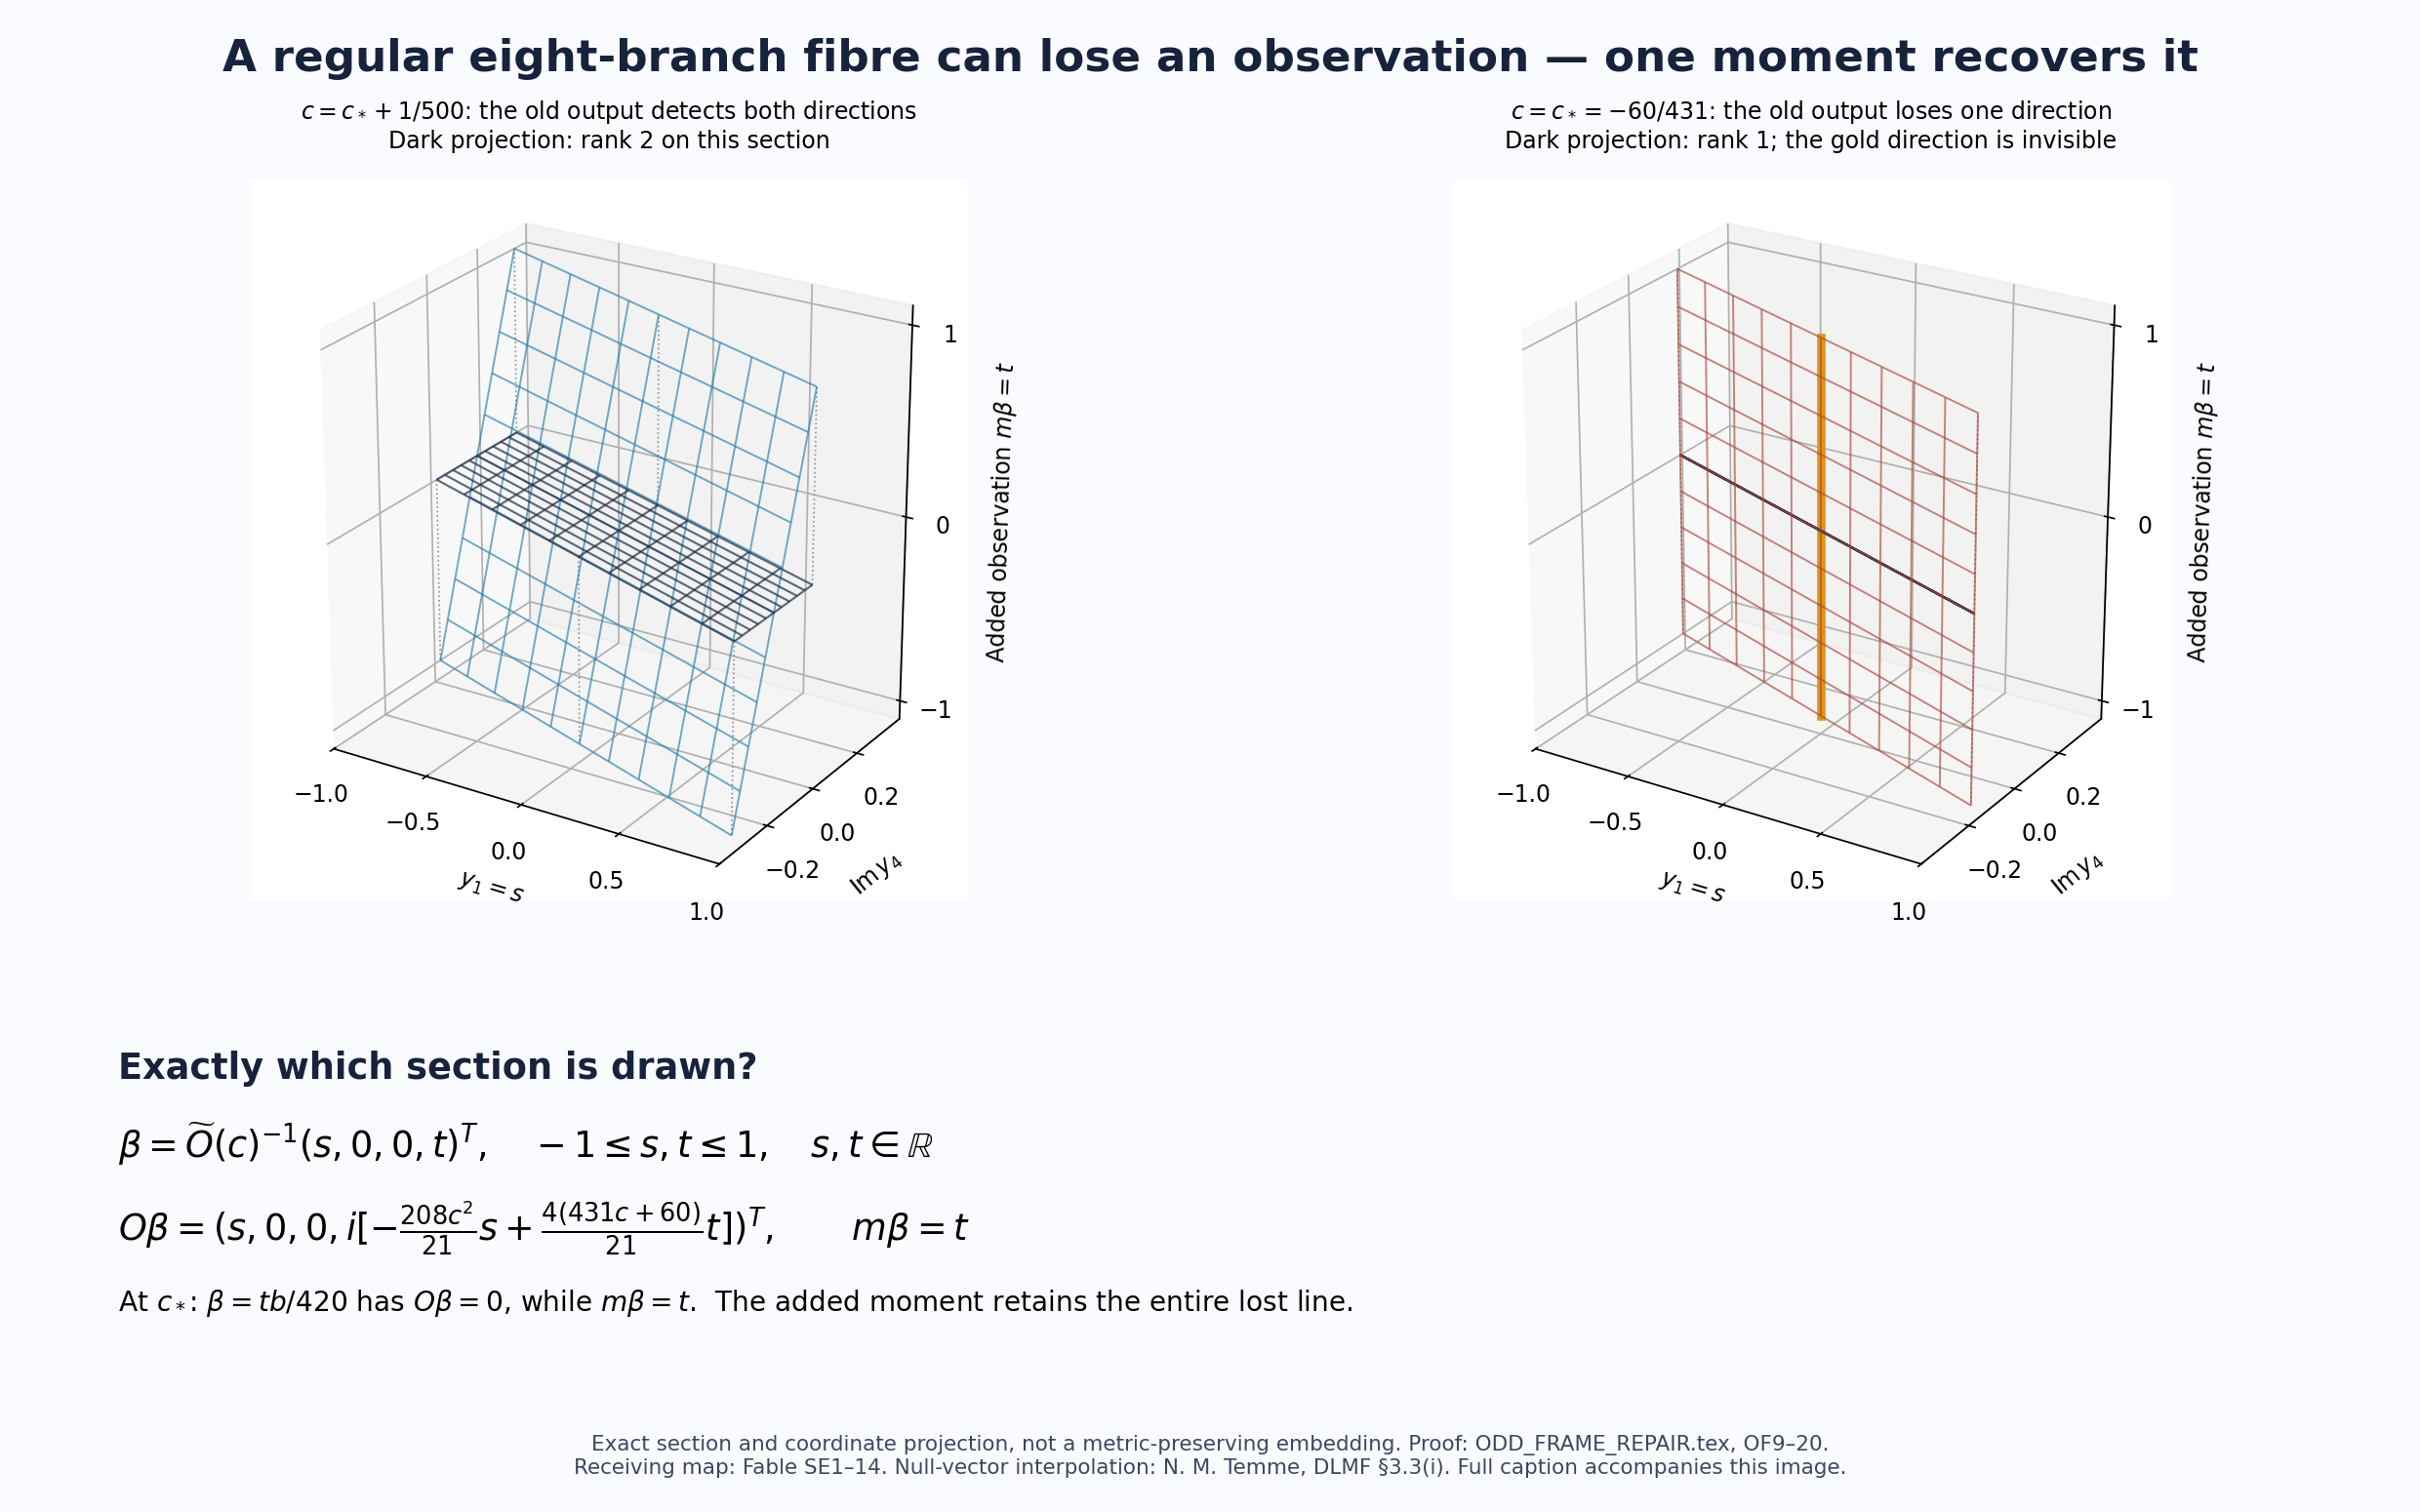
\includegraphics[width=\linewidth]{ODD_FRAME_REPAIR_ILLUSTRATION.png}
\caption{An exact section of the receiving map and its repair. For
$\beta=\widetilde O(c)^{-1}(s,0,0,t)^T$, with real $s,t\in[-1,1]$,
the drawn coordinates are
$(y_1,\operatorname{Im}y_4,m\beta)
=(s,-208c^2s/21+4(431c+60)t/21,t)$.
Both targets have four simple roots. The dark coordinate projection
forgets the added cubic moment. It has rank two on the left, but
rank one at $c_*=-60/431$ on the right. The gold line is
$\beta=tb/420$; its original output is zero and its added moment
is $t$. OF9--20 prove the exact inverse, minimal repair and original
two-Gram return. This is a coordinate section, not an isometric
embedding of the Gamma norm. Receiving columns: \cite[SE1--14]{sfrepair:Fable};
classical null-vector interpolation: \cite[3.3(i)]{sfrepair:Temme}; received
divisor and repair: \cite{sfrepair:Incoming}.}
\end{figure}
\clearpage
\begin{thebibliography}{9}
\bibitem{sfrepair:Fable} Split-Zero programme, \emph{Fable to the original
conductor}, source \texttt{FABLE\_TO\_ORIGINAL\_CONDUCTOR.tex},
consulted source hash
\nolinkurl{9629ec8ff32c069a7329c012687fd8bcfd7d5c9437a94fcfba1d4725edbec764}.
GF20--21, SE1--14 and RW14--19 are the exact receiving passages used.
\url{https://github.com/KokunoYumeto/zeta-function-research-reader}.
This programme source records the underlying human-source provenance
of the original polynomial separately; the receiving divisor and
repair here are attributed to the received continuation below.
\bibitem{sfrepair:Incoming} User-supplied web-session calculation,
\emph{The relevant strand is Erd\H{o}s--Straus/Fable},
received 20 September 2026; no human author name supplied.
Original SHA256
\nolinkurl{57efa66b73bb4ce951b1d17ec4170b0f7bf1a00af3718e56faa71e7693ec2717}.
Equations (1)--(28) supply the divisor, pole and proposed repair;
OF19--22 articulate its full even-coordinate return and evaluate
the finite inverse coefficient. Original input remains preserved
in the private source register.
\bibitem{sfrepair:Temme} N.~M.~Temme, \emph{Numerical Methods}, NIST Digital
Library of Mathematical Functions, version 1.2.8, section 3.3(i),
equations 3.3.1, 3.3.2, 3.3.3 and 3.3.3\_1,
\url{https://dlmf.nist.gov/3.3.i}.
Original equation TeX read and retained. The DLMF source notes cite
P.~J.~Davis, \emph{Interpolation and Approximation} (1975),
pages 56 and 67--68; this note consulted the original DLMF equations,
not that entire book. OF8 gives the full proof of the specialization.
\end{thebibliography}

\endgroup

\clearpage\begingroup
\part*{Complete signed-orbit reconstruction and the two original metrics}
\newcommand{\sforbitC}{\mathbb C}
\newcommand{\sforbittr}{\operatorname{tr}}
\newcommand{\sforbitdiag}{\operatorname{diag}}
\newcommand{\sforbitsgn}{\operatorname{sgn}}
\newcommand{\sforbitrank}{\operatorname{rank}}
\newcommand{\sforbitim}{\operatorname{im}}
\newcommand{\sforbiteps}{\varepsilon}
\newcommand{\sforbitone}{\mathbf 1}



\paragraph{Scope and correction.}
This note proves the finite-orbit formulas in Sections 5--6 of the
received calculation \cite{sforbit:Incoming}, and carries their metric calculation
through the original two receiving maps.  Its group formulas (31)--(38)
are valid with a positive quotient metric.  Its equations (40)--(44)
use a specified equal-Gram metric.  The original target has instead
the two coordinate Grams $(G_Y,G)$, and the original source has
$(G_X,G_U)$, as displayed in SE13, TC9, RW14 and RW19 of \cite{sforbit:Fable}.
We prove the exact formulas for those original metrics below; equality
of the two Grams is neither required nor inferred.
All root labels, inverse-square-root phases and powers of the boundary
parameter are retained.

\section{Literal states and the finite group}
Let
\[
 h(r)=Ar^4+r^3+Br^2+Cr+D,\qquad A\ne0,
 \tag{OM1}
\]
have four distinct complex roots $r_1,\ldots,r_4$, in a fixed order.
Put $d_j=h'(r_j)$, and fix one of the two choices
$\xi_j^2d_j=1$ at each root.  The two original inverse states over
root $r_j$ are $p_j^\pm=e_j\pm o_j$, where
\[
e_j=\begin{pmatrix}
0\\-r_j\\3id_j\\(B-17r_j+Ar_j^2)d_j-2Ad_j^2
\end{pmatrix},\quad
o_j=\xi_j\begin{pmatrix}
1\\-id_j\\Ad_j^2+2r_jd_j\\i(7r_j^2d_j-13d_j^2)
\end{pmatrix}.
\tag{OM2}
\]
These are the coefficient vectors from \cite{sforbit:Incoming}, equation (1);
they are used literally throughout.  Set $E=[e_1\ \cdots\ e_4]$,
$O=[o_1\ \cdots\ o_4]$, $S=[E\ O]$ and
$V=\sforbitC^4_\alpha\oplus\sforbitC^4_\beta$.  For original branch coefficients
$c_j^\pm$ the exact coordinate maps are
\[
\alpha_j=c_j^++c_j^-,\quad \beta_j=c_j^+-c_j^-,
\qquad c_j^\pm=\tfrac12(\alpha_j\pm\beta_j),
\qquad \sum_{j,\pm}c_j^\pm p_j^\pm=S(\alpha,\beta).
\tag{OM3}
\]
In particular $\|\alpha\|_2^2+\|\beta\|_2^2=
2\sum_j(|c_j^+|^2+|c_j^-|^2)$.  Euclidean coefficient norms below
refer to the displayed $(\alpha,\beta)$ coordinates, with this factor
retained when returning to the $c^\pm$ coordinates.

Write $P_\pi e_j=e_{\pi(j)}$ and $D_\sforbiteps=\sforbitdiag(\sforbiteps_1,\ldots,\sforbiteps_4)$.
The finite group and its representation are
\[
\mathcal G=\{(\sforbiteps,\pi):\sforbiteps_j\in\{1,-1\},
       \ \prod_j\sforbiteps_j=\sforbitsgn\pi\},\qquad
R_{\sforbiteps,\pi}=\sforbitdiag(P_\pi,D_\sforbiteps P_\pi).
\tag{OM4}
\]
Here the signs $\sforbiteps$ label output coordinates; a convention in which
they label input roots is converted by $\sforbiteps_{\pi(j)}=\sigma_j$.
This states the exact relation to SM4--6 of \cite{sforbit:Fable}.
The product is
$(\sforbiteps,\pi)(\delta,\sigma)=(\sforbiteps\,(\pi\delta),\pi\sigma)$, with
$(\pi\delta)_j=\delta_{\pi^{-1}(j)}$.  Its sign product is
$\sforbitsgn(\pi)\sforbitsgn(\sigma)$, so it remains in $\mathcal G$, and direct
matrix multiplication proves that $R$ is a representation.  There
are eight sign vectors for each of the twenty-four permutations:
$|\mathcal G|=192$.

\section{Exact averaging and reconstruction}
Let $G$ be a fixed positive Hermitian Gram on the receiving coefficient
space $\sforbitC^4$.  Define
\[
P_0=\tfrac14\sforbitone\sforbitone^*,\quad P_3=I-P_0,\qquad
\lambda_0=\tfrac14\sforbitone^*E^*GE\sforbitone,\quad
\lambda_3=\frac{\sforbittr(E^*GE)-\lambda_0}{3},\quad
\lambda_4=\tfrac14\sforbittr(O^*GO).
\tag{OM5}
\]
Then
\[
\frac1{192}\sum_{g\in\mathcal G}R_g^*S^*GS R_g
=D_\lambda:=
\sforbitdiag(\lambda_0P_0+\lambda_3P_3,\lambda_4I_4).
\tag{OM6}
\]
Here is a direct proof of every coefficient.  For fixed $\pi$, the
admissible signs have prescribed product $\sforbitsgn\pi$.  The average of
$\sforbiteps_i$ is zero: flipping $i$ and any other coordinate is a
sign-product-preserving involution reversing it.  For $i\ne j$,
the average of $\sforbiteps_i\sforbiteps_j$ is zero by flipping $i$ and a coordinate
outside $\{i,j\}$.  Thus averaging $D_\sforbiteps C D_\sforbiteps$ keeps exactly
the diagonal of $C$, and averaging any entry of $B D_\sforbiteps$ gives
zero.  The mixed blocks of $S^*GS$ vanish under this sign average.
The odd diagonal entries then average under all permutations to
$\sforbittr(O^*GO)/4$.

For completeness let $A_0=E^*GE$.  The average of $P_\pi^*A_0P_\pi$
has constant diagonal $\sforbittr(A_0)/4$ and constant off-diagonal
$\sum_{i\ne j}(A_0)_{ij}/12$.  It therefore has eigenvalue
$\sforbitone^*A_0\sforbitone/4$ on $\sforbitC\sforbitone$ and eigenvalue
$(\sforbittr A_0-\sforbitone^*A_0\sforbitone/4)/3$ on $\sforbitone^\perp$.
This is precisely the even block of OM6.  The argument applies
equally to the even and odd sign cosets; averaging only the
even signs at an odd permutation would not enumerate $\mathcal G$.

Every $\lambda$ in OM5 is strictly positive, including at a singular
odd receiving matrix.  To retain quantitative bounds, a coordinate
covector satisfies
\[
|v_k|^2\le (G^{-1})_{kk}\,v^*Gv.
\tag{OM7}
\]
Indeed this is Cauchy--Schwarz applied to $G^{-1/2}e_k$ and
$G^{1/2}v$.  Since $\sum_jr_j=-1/A$, the second row of $E\sforbitone$
is $1/A$.  Further,
$3\lambda_3=\sforbittr(P_3E^*GE P_3)$, whose columnwise second coordinates
are $-(r_j-r_{\rm av})$, where $r_{\rm av}=-1/(4A)$.
The first coordinates of $O$ are $\xi_j$, with
$|\xi_j|^2=1/|d_j|$.  Applying OM7 gives
\[
\lambda_0\ge\frac1{4|A|^2(G^{-1})_{22}},\quad
\lambda_3\ge
\frac{\sum_j|r_j-r_{\rm av}|^2}{3(G^{-1})_{22}},\quad
\lambda_4\ge\frac{\sum_j|d_j|^{-1}}{4(G^{-1})_{11}}.
\tag{OM8}
\]
Distinct roots make the middle numerator positive.  No determinant
of $O$ occurs in this proof.

The orbit observation is the explicitly defined map
\[
\mathcal T:V\longrightarrow(\sforbitC^4)^{\oplus192},\qquad
(\mathcal Tv)_g=S R_gv,
\tag{OM9}
\]
where the codomain has Gram $G^{\oplus192}$.  Its adjoint, with the
ordinary coefficient Gram on $V$, is
$\mathcal T^\dagger y=\sum_g R_g^*S^*G y_g$.
OM6 gives $\mathcal T^\dagger\mathcal T=192D_\lambda$ and hence
\[
v=\frac1{192}D_\lambda^{-1}\sum_gR_g^*S^*G(\mathcal Tv)_g.
\tag{OM10}
\]
Define $\mathcal L=(192D_\lambda)^{-1}\mathcal T^\dagger$.
Then
$\mathcal L\mathcal L^\dagger=(192D_\lambda)^{-1}$, so its exact
operator norm is
\[
\|\mathcal L\|_{G^{\oplus192}\to2}
=[192\min(\lambda_0,\lambda_3,\lambda_4)]^{-1/2}.
\tag{OM11}
\]
This proves the incoming noise bound and its sharp constant.
The data in OM9 are all 192 displayed observations.  OM10 is not
an identification of this data space with one observation at one
fixed arithmetic parameter.

\section{The actual quotient observation and its entire kernel}
Retain the original coefficient map $\Psi:\sforbitC^4\to W$, the original
observation $\Lambda_W:W\to B$, and its actual positive quotient
Gram $Q$ on $B$.  Put
\[
Z=\Lambda_W\Psi,\quad G_\Lambda=Z^*QZ,\quad
(\mathcal T_\Lambda v)_g=ZS R_gv.
\tag{OM12}
\]
No positive definiteness of $G_\Lambda$ is assumed: it is the
pullback of the original quotient metric.  Substitution in OM5--6
gives exactly
\[
\begin{split}
\lambda_{\Lambda,0}&=\tfrac14\|ZE\sforbitone\|_Q^2,\\
\lambda_{\Lambda,3}&=\tfrac13\sum_j\|ZE P_3e_j\|_Q^2,\\
\lambda_{\Lambda,4}&=\tfrac14\sum_j\|ZO e_j\|_Q^2,\\
\mathcal T_\Lambda^\dagger\mathcal T_\Lambda
&=192\sforbitdiag(\lambda_{\Lambda,0}P_0+
\lambda_{\Lambda,3}P_3,\lambda_{\Lambda,4}I_4).
\end{split}\tag{OM13}
\]
The exact whole kernel therefore is the direct sum of those of the
following three spaces for which the displayed test vanishes:
\[
\begin{array}{c|c|c}
\text{space}&\text{dimension}&\text{vanishing test}\\ \hline
\sforbitC\sforbitone\oplus0&1&ZE\sforbitone=0\\
\sforbitone^\perp\oplus0&3&ZE P_3=0\\
0\oplus\sforbitC^4&4&ZO=0 .
\end{array}\tag{OM14}
\]
Indeed the squared norm of $\mathcal T_\Lambda v$ is the sum of
three nonnegative terms in OM13.  A term vanishes on its whole
component exactly when its coefficient is zero.  As $Q$ is
positive on the attained quotient, a sum of its squared norms
vanishes exactly when every indicated vector vanishes.
If a different presentation retains a semidefinite $Q$, the tests
must instead be made after $Q^{1/2}$; OM13 itself still holds.

This also gives an explicit reconstruction of all surviving states,
without a missing injectivity assumption.  In $D_{\Lambda}^{+}$
replace each positive $\lambda_{\Lambda,j}$ by its inverse and each
zero one by zero, keeping the same $P_0,P_3,I_4$ blocks.  Then
\[
\frac1{192}D_\Lambda^+
\sum_gR_g^*S^*Z^*Q(\mathcal T_\Lambda v)_g
=\sforbitdiag(\chi_0P_0+\chi_3P_3,\chi_4I_4)v,
\quad
\chi_j=\begin{cases}1&\lambda_{\Lambda,j}>0,\\0&\lambda_{\Lambda,j}=0.
\end{cases}
\tag{OM15}
\]
This is a direct multiplication using OM13, not an unevaluated
choice of a section.  Its image is the Euclidean orthogonal
complement of the exact kernel OM14.  Its noise norm on the
nonzero image is the reciprocal square root of $192$ times the
smallest positive $\lambda_{\Lambda,j}$.  If all vanish, the
receiver is the zero map, as OM15 states.

\paragraph{An evaluated nonzero observation at the new divisor.}
The regular target $(A,B,C,D)=(1,0,c_*,0)$, $c_*=-60/431$, permits
a concrete test of OM14.  Take the explicitly specified scalar
observation
\[
Z=\ell^T=(208c_*^2,\,5ic_*,\,60,\,-21i),\qquad Q=1.
\tag{OM16}
\]
This is a test observation on the receiving coefficient space;
it is not being substituted for the programme's given $\Lambda_W\Psi$.
With $h=r^4+r^3+c_*r$ and $d=4r^3+3r^2+c_*$, reduction of
\[
208c_*^2+5c_*d+60(d^2+2rd)+21(7r^2d-13d^2)
\]
modulo $h$ is zero.  Thus $\ell^TO=0$ for every fixed choice of
the square-root phases.  Reduction of $\ell^T e(r)/i$ gives
\[
f(r)=\frac{60}{185761}
 (1073621r^3+1680900r^2+490909r-75060).
\tag{OM17}
\]
These two reductions are polynomial identities; they follow by
substituting $r^4=-r^3-c_*r$ until degree at most three remains.
To evaluate squared norms without unproved conjugation assumptions,
all four roots are real.  The cubic $r^3+r^2+c_*$ is negative at
$0$, positive at $-2/3$ (its value is $104/11637$), tends to
$-\infty$ at $-\infty$ and to $+\infty$ at $+\infty$.
Its derivative $r(3r+2)$ is nonzero in each of the three open
intervals between these extrema, so it has three distinct real
roots; the fourth root $0$ of $h$ is distinct.

The sums $p_k=\sum_jr_j^k$ are, for $0\le k\le6$,
\[
\left(4,-1,1,-\frac{251}{431},\frac{191}{431},
             -\frac{131}{431},\frac{41401}{185761}\right).
\tag{OM18}
\]
The first three follow from the elementary symmetric coefficients,
$p_3=-1-3c_*$, and for $k\ge4$ the equation of each root gives
$p_k=-p_{k-1}-c_*p_{k-3}$.  Expanding OM17 and its square using
these values gives
\[
\sum_jf(r_j)=\frac{15870600}{185761},\qquad
\sum_jf(r_j)^2=\frac{348296871672000}{34507149121}.
\tag{OM19}
\]
Since $\ell^Te_j=if(r_j)$, OM13 now evaluates to
\[
\lambda_{\Lambda,0}=\frac{62968986090000}{34507149121},
\qquad
\lambda_{\Lambda,3}=\frac{95109295194000}{34507149121},
\qquad
\lambda_{\Lambda,4}=0.
\tag{OM20}
\]
Consequently this nonzero scalar observation has a complete-orbit
map of rank exactly four: it recovers every even state and kills
the entire odd sector.  The fixed observation has rank one, whereas
the displayed 192-coordinate observation has rank four; OM13--15
prove the exact map relating those statements.

\section{The original two-Gram metric}
Let $H>0$ be the label-coordinate Gram and $G>0$ the
evaluation-coordinate Gram.  The coefficient map and its pullback
are
\[
J=\begin{pmatrix}I&0\\E&O\end{pmatrix},\qquad
M_{H,G}=J^*\sforbitdiag(H,G)J
=\begin{pmatrix}H+E^*GE&E^*GO\\O^*GE&O^*GO\end{pmatrix}.
\tag{OM21}
\]
The exact original receiving maps are
\[
\mathcal J_W(\alpha,\beta)
 =(Y\alpha,\Psi(E\alpha+O\beta)),\quad
\mathcal J_U(\alpha,\beta)
 =(X\alpha,\Phi(E\alpha+O\beta)).
\tag{OM22}
\]
Thus their original orthogonal direct-sum norms give respectively
\[
(H,G)=(G_Y,G)\quad\hbox{and}\quad(H,G)=(G_X,G_U),
\tag{OM23}
\]
where $G_Y=Y^*\langle\, ,\,\rangle_{\Gamma,W}Y$ and
$G=\Psi^*\langle\, ,\,\rangle_{\Gamma,W}\Psi$, and the source
uses the actual quotient metric in both source copies.  Further,
$T_AX=Y$ and $T_A\Phi=\Psi$ prove the full commuting identity
$(T_A\oplus T_A)\mathcal J_U=\mathcal J_W$ by substitution.
This retains the exact morphism between both original metrics.
No equality of $G_Y$ with $G$, or of $G_X$ with $G_U$, is implied.

In the remainder of this section $O$ is invertible, so that $M_{H,G}$
is positive definite.  This holds on the punctured boundary in
the next section.  At the regular-target odd-frame divisor, the
same matrix is semidefinite with its actual kernel; the positive
comparison problem below is not asserted there.
Put
\[
A_0=H+E^*GE,\quad B_0=O^*GO,\quad C_0=E^*GO,\qquad
\zeta_{H,G}=\|G^{1/2}EH^{-1/2}\|_2 .
\tag{OM24}
\]
Among all positive block-diagonal forms $K=\sforbitdiag(K_e,K_o)$,
the exact least relative comparison ratio is
\[
\inf_{\substack{K>0\ {\rm block\ diagonal},\ 0<\alpha\le\beta\\
                 \alpha M_{H,G}\preceq K\preceq\beta M_{H,G}}}
\frac{\beta}{\alpha}
=\bigl(\sqrt{1+\zeta_{H,G}^2}+\zeta_{H,G}\bigr)^2.
\tag{OM25}
\]
The infimum is attained.  To prove this, the invertible block
congruence $\sforbitdiag(A_0^{-1/2},B_0^{-1/2})$ carries $M_{H,G}$ to
$\begin{psmallmatrix}I&T\\T^*&I\end{psmallmatrix}$, where
$T=A_0^{-1/2}C_0B_0^{-1/2}$.  This congruence is used solely
to prove the comparison and is inverted below; it does not
replace either original norm.  The matrix
$U=G^{1/2}OB_0^{-1/2}$ is unitary, so
\[
TT^*=A_0^{-1/2}E^*GEA_0^{-1/2},\qquad
\eta:=\|T\|_2=\frac{\zeta_{H,G}}{\sqrt{1+\zeta_{H,G}^2}}.
\tag{OM26}
\]
For the second equality, the eigenvalues of the first matrix are
the generalized eigenvalues of $(E^*GE,H+E^*GE)$.
An eigenvector of $H^{-1/2}E^*GEH^{-1/2}$ with eigenvalue
$s^2$ gives generalized eigenvalue $s^2/(1+s^2)$, and these
vectors form a basis.  Its largest $s$ is $\zeta_{H,G}$.

Choose unit singular vectors $x,y$ with $x^*Ty=\eta$ real
nonnegative.  The vectors $(x,y)$ and $(x,-y)$ have equal
norm in every block-diagonal form, but their squared norms in
the transformed $M_{H,G}$ are $2+2\eta$ and $2-2\eta$.
Consequently any comparison satisfies
$\beta/\alpha\ge(1+\eta)/(1-\eta)$.
Conversely the identity matrix in these coordinates satisfies
the comparison with
$\alpha=1/(1+\eta)$ and $\beta=1/(1-\eta)$:
the eigenvalues of the transformed $M_{H,G}$ are $1\pm s_j(T)$.
Returning to the original coordinates, this identity matrix is
$K=\sforbitdiag(A_0,B_0)$.  It attains the lower bound.
Finally $(1+\eta)/(1-\eta)=
(\sqrt{1+\zeta_{H,G}^2}+\zeta_{H,G})^2$, proving OM25.

Finite-group averaging of the full original form is also exact:
\[
\overline M_{H,G}
 :=\frac1{192}\sum_gR_g^*M_{H,G}R_g
 =\sforbitdiag(\mu_0P_0+\mu_3P_3,\mu_4I_4),
\tag{OM27}
\]
where
\[
\mu_0=\tfrac14\sforbitone^*(H+E^*GE)\sforbitone,\quad
\mu_3=\frac{\sforbittr(H+E^*GE)-\mu_0}{3},\quad
\mu_4=\tfrac14\sforbittr(O^*GO).
\tag{OM28}
\]
This follows from the entrywise sign and permutation sum already
proved in OM6, applied to the three blocks of OM21.  In particular
\[
\det\overline M_{H,G}=\mu_0\mu_3^3\mu_4^4,\qquad
\det M_{H,G}=|\det O|^2\det H\det G.
\tag{OM29}
\]
The second identity uses $\det J=\det O$ and multiplication of
determinants in the exact congruence OM21.

\section{Original escaping boundary, with all leading constants}
Fix $B,C,D$, assume the cubic $r^3+Br^2+Cr+D$ is squarefree
and $\Delta_0:=3C-B^2\ne0$, and vary $A=t\to0$.
Fix the label and evaluation Grams $H,G$ in OM21; the auxiliary
Fable polynomial varies while those original receiving maps
and their physical metrics are held fixed.
Exactly three roots remain bounded: the implicit-function theorem
at each simple cubic root supplies those analytic branches.
For the fourth root, set $v=1/r$.  Its equation is
$t+v+Bv^2+Cv^3+Dv^4=0$, whose derivative with respect to $v$
at $(t,v)=(0,0)$ is one.  Thus
\[
v=-t-Bt^2+O(t^3),\quad
r_\infty=-t^{-1}+B+O(t),\quad
d_\infty=-t^{-2}+4Bt^{-1}+O(1).
\tag{OM30}
\]
An analytic inverse square root on a small punctured disk is
$\xi_\infty=it(1+2Bt+O(t^2))$; the opposite choice negates
the odd column, and does not change any ensuing Gram constant.
Substitution in every coordinate of OM2 gives
\[
e_\infty=-20t^{-3}e_4+O(|t|^{-2}),\qquad
o_\infty=20t^{-3}e_4+O(|t|^{-2}).
\tag{OM31}
\]
For the fourth mean coordinate, the two leading contributions
are $18t^{-1}(-t^{-2})$ and $-2t(t^{-4})$.
For the fourth odd coordinate, $7r_\infty^2d_\infty-
13d_\infty^2=-20t^{-4}+O(t^{-3})$, multiplied by
$i\xi_\infty=-t+O(t^2)$.  The remaining coordinates have
smaller pole order, and the other three columns are bounded.
This proves the constants and phases in OM31.

Let $j_\infty$ be the fixed label of this column.
The rank-one leading matrix gives
\[
E=-20t^{-3}e_4e_{j_\infty}^T+O(|t|^{-2}),\qquad
\zeta_{H,G}
=20\sqrt{G_{44}(H^{-1})_{j_\infty j_\infty}}\,
 |t|^{-3}(1+O(|t|)).
\tag{OM32}
\]
The operator norm of a rank-one matrix $uv^*$ is
$\|u\|_2\|v\|_2$, which gives the coefficient here.
The norm is Lipschitz in the matrix entries, so the matrix
remainder yields the stated relative remainder.  Since
$(\sqrt{1+z^2}+z)^2=4z^2(1+O(z^{-2}))$ for real $z\to\infty$,
OM25 becomes
\[
\boxed{\inf\frac{\beta}{\alpha}
=1600G_{44}(H^{-1})_{j_\infty j_\infty}
 |t|^{-6}(1+O(|t|)).}
\tag{OM33}
\]

For a self-contained determinant calculation at this boundary,
reduce the four polynomial components of $o_j/\xi_j$ modulo
$h$, using $r^4=-(r^3+Br^2+Cr+D)/t$.
The constant first row leaves the following determinant after
the factors $-i$ and $i$ cancel:
\[
\mathsf R(t)=\begin{pmatrix}
2B&3&4t\\
4tBC-8tD-7C&4tB^2-2tC-16t^2D-5B&4tB-8t^2C-3\\
20C/t+76D-52BC&20B/t+5C-52B^2+208tD&20/t-66B+104tC
\end{pmatrix}.
\tag{OM34}
\]
Every entry is a coefficient in the unchanged power basis
$1,r,r^2,r^3$.  Expansion of its leading term gives
\[
\det\mathsf R(t)
=\frac{20}{t}
\det\begin{pmatrix}2B&3&0\\-7C&-5B&-3\\sforbitC&B&1\end{pmatrix}
 +O(1)
=\frac{80(3C-B^2)}t+O(1).
\tag{OM35}
\]
If $V_r=\prod_{j<k}(r_k-r_j)$, then
$\prod_jd_j=t^4V_r^2$.  Hence
$(V_r\prod_j\xi_j)^2=t^{-4}$ and
$V_r\prod_j\xi_j=\sforbiteps_{\rm br}t^{-2}$ for a locally fixed
$\sforbiteps_{\rm br}\in\{1,-1\}$.  Evaluation of the reduced
coefficient matrix at the four roots therefore proves
\[
\det O=\sforbiteps_{\rm br}t^{-2}\det\mathsf R(t),\qquad
|\det O|^2=6400|\Delta_0|^2|t|^{-6}(1+O(|t|)).
\tag{OM36}
\]
As $\Delta_0\ne0$, $O$ is invertible for every sufficiently small
nonzero $t$; thus the positivity assumption used in OM25 has
been established on this boundary.

The same single escaping column in OM31 gives
\[
\mu_0=100G_{44}|t|^{-6}(1+O(|t|)),\quad
\mu_3=100G_{44}|t|^{-6}(1+O(|t|)),\quad
\mu_4=100G_{44}|t|^{-6}(1+O(|t|)).
\tag{OM37}
\]
In detail the leading terms of $\sforbittr E^*GE$ and
$\sforbitone^*E^*GE\sforbitone$ are both $400G_{44}|t|^{-6}$;
division by four gives the first coefficient, and
$(400-100)/3=100$ gives the second.
The odd trace has the same leading coefficient.  The fixed
entries of $H$ have lower order and remain in OM28.
Multiplication of all eight factors in OM29, followed by OM36,
proves
\[
\boxed{\frac{\det\overline M_{H,G}}{\det M_{H,G}}
=\frac{100^8G_{44}^8}
 {6400|3C-B^2|^2\det H\det G}
 |t|^{-42}(1+O(|t|)).}
\tag{OM38}
\]
The numerator grows with order $48$, and the denominator grows
with order $6$.  This proves the exact exponent $42$ and its
coefficient without imposing group invariance on the old metric.

\paragraph{Back to the two original sides.}
Equations OM23, OM33 and OM38 give the complete target constants
\[
1600G_{44}(G_Y^{-1})_{j_\infty j_\infty},\qquad
\frac{100^8G_{44}^8}
 {6400|3C-B^2|^2\det G_Y\det G},
\tag{OM39}
\]
and the complete source constants
\[
1600(G_U)_{44}(G_X^{-1})_{j_\infty j_\infty},\qquad
\frac{100^8(G_U)_{44}^8}
 {6400|3C-B^2|^2\det G_X\det G_U}.
\tag{OM40}
\]
The corresponding exponents are $-6$ and $-42$ in each case.
The incoming equal-Gram formulas follow exactly by setting
$H=G$ in OM33 and OM38, as the explicitly defined metric in
its equation (40) does.  For the actual programme target and
source, OM39--40 retain the distinct original label Grams.
No estimate of a Hermitian norm in this note assigns a
phase-sensitive arithmetic current sign.

\begin{thebibliography}{9}
\bibitem{sforbit:Incoming}
User-supplied AI web-session calculation,
\emph{The relevant strand is Erd\H{o}s--Straus/Fable},
received 20 September 2026, equations (1)--(44).
No author name was supplied.
The exact incoming file has SHA-256
\path{57efa66b73bb4ce951b1d17ec4170b0f7bf1a00af3718e56faa71e7693ec2717}.
Its original pinned working-source commit is
\path{ab45e221579a0d48ce2885b4ecdf1a6aefc24a20}.
This note reads its entire text and independently proves the
orbit and metric claims; it corrects the native metric identification.

\bibitem{sforbit:Fable}
Split-Zero programme,
\emph{Fable to the original conductor: Inverse branches, signed
states, and boundary action},
\texttt{FABLE\_TO\_ORIGINAL\_CONDUCTOR.tex},
accepted local source snapshot, 20 September 2026.
Exact snapshot SHA-256
\path{9629ec8ff32c069a7329c012687fd8bcfd7d5c9437a94fcfba1d4725edbec764}.
The exact sections read for this derivation are SE11--18,
SM3--7, TC8--9 and RW14--20, together with the bibliography.
Repository:
\url{https://github.com/KokunoYumeto/zeta-function-research-reader}.
The source attributes the original marked polynomial to
The Clankers' Erd\H{o}s--Straus reader and the preceding
Alp\"oge--Fable example to the human sources retained there.
Those original publications are not represented as independently
read in this derivation.  The finite averaging, exact kernel,
comparison optimization and boundary constants used here have
complete algebraic proofs above; no unquoted human theorem is
being imported to justify them.
\end{thebibliography}

\endgroup

\clearpage\begingroup
\part*{The original arithmetic secular determinant and its full pole cancellation}
\newcommand{\sfsecC}{\mathbb C}\newcommand{\sfsecR}{\mathbb R}
\newcommand{\sfsecPP}{\mathcal P}\newcommand{\sfsecId}{\operatorname{Id}}
\newcommand{\sfsectr}{\operatorname{tr}}\newcommand{\sfsecim}{\operatorname{im}}
\newcommand{\sfsecord}{\operatorname{ord}}
\newtheorem{sfsectheorem}{Theorem}[section]
\newtheorem{sfsecproposition}[sfsectheorem]{Proposition}
\newtheorem{sfseclemma}[sfsectheorem]{Lemma}


\section{The original arithmetic source and every coordinate}

This is a finite-parameter sequel to the native polynomial calculation
\cite{sfsec:Native}. Its human-source comparison is the finite rank-one
determinant calculation of Connes--Consani--Moscovici \cite{sfsec:CCM},
Lemma \texttt{key} and equation \texttt{eq:detDp}.
Every determinant below is a finite determinant. No regularized
infinite determinant or convergence of spectra is inferred.
No conclusion that every root of the original arithmetic
annihilator lies on $\Re S=c$ is inferred.

Retain the actual finite divisor and source
\begin{equation}\tag{NS1}\label{sfsec:NS1}
h(s)=\prod_{\rho\in Z}(s-\rho)^{m_\rho},\qquad
g(s)=2\xi(s)=s(s-1)\pi^{-s/2}\Gamma(s/2)\zeta(s),\qquad
\mathcal M F_h=g/h.
\end{equation}
Here $Z$ is the original nonempty set of actual nontrivial zeros,
closed under conjugation and $s\mapsto1-s$, with every complete
order $m_\rho$. This refers to the specified packet, not to the
existence of any off-line zero. The original Mellin convention is
$\mathcal M F(s)=\int_0^\infty F(x)x^{s-1}\,dx$ and $D=-x\partial_x$.
For its actual tensor degree $k\geq1$, put
\begin{equation}\tag{NS2}\label{sfsec:NS2}
\begin{gathered}
c=k/2,\qquad S=c+iu,\qquad
w_h(t)=\frac{|(g/h)(1/2+it)|^2}{2\pi},\qquad m=w_h^{*k},\\
\mu_h=\int_\sfsecR w_h(t)\,dt,\qquad
\int_\sfsecR m(u)\,du=\mu_h^k=:\mathfrak m,\\
\mathcal A P=P(D_1+\cdots+D_k)F_h^{\otimes k},\qquad
\langle\mathcal A P,\mathcal A Q\rangle
 =\int_\sfsecR\overline{P(c+iu)}Q(c+iu)m(u)\,du .
\end{gathered}
\end{equation}
The last equality follows by Mellin Parseval on each original
$dx_j$ axis and by the convolution definition. In particular
$\|\mathcal A1\|^2=\mathfrak m$, not one.
The entire quotient $g/h$ is nonzero, so its isolated zeros make
$w_h$ positive almost everywhere. It is even by conjugation.
The vertical Gamma bound and the alternating-series integral for
$\zeta$ give a polynomial times $e^{-\pi|t|/2}$ for $w_h$ outside
a compact interval; the removable values of $g/h$ are bounded on
that interval. Thus all its moments exist, as do those of $m$.
Convolution preserves evenness and positivity almost everywhere.
Every nonzero polynomial therefore has positive squared norm.

Let $Q_n$ be the real monic orthogonal polynomials for this very
measure, with full norms
\begin{equation}\tag{NS3}\label{sfsec:NS3}
\begin{gathered}
\omega_n=\int_\sfsecR Q_n(u)^2m(u)\,du>0,\qquad
\omega_0=\mathfrak m,\qquad a_n=\sqrt{\omega_{n+1}/\omega_n},
\quad a_{-1}=0,\\
\phi_n=Q_n/\sqrt{\omega_n},\qquad
p_n(S)=i^nQ_n((S-c)/i),\\
u\phi_n=a_{n-1}\phi_{n-1}+a_n\phi_{n+1},
\qquad Q_n(-u)=(-1)^nQ_n(u).
\end{gathered}
\end{equation}
Gram--Schmidt supplies the unique monic $Q_n$. Uniqueness after
$u\mapsto-u$ proves parity. Pairing $uQ_n$ with earlier
polynomials kills all terms below $Q_{n-1}$; parity kills the
$Q_n$ term; the leading coefficient and the $Q_{n-1}$ pairing
give the displayed recurrence. This proves the formulas without
substituting a comparison measure.

The exact original cyclic annihilator is
\begin{equation}\tag{NS4}\label{sfsec:NS4}
\begin{gathered}
\chi(S)=\prod_\kappa(S-\kappa)^{e_\kappa},\qquad
e_\kappa=\max_{\rho_1+\cdots+\rho_k=\kappa}
 \left(1+\sum_{j=1}^k(m_{\rho_j}-1)\right),\\
q=\deg\chi,\qquad C=\sfsecC[S]/(\chi),\qquad
M=\frac{M_S-cI}{i},\qquad
\chi_u(z)=i^{-q}\chi(c+iz)=\det(zI-M).
\end{gathered}
\end{equation}
To prove the exponent formula, the local factor of
$(\sfsecC[s]/h)^{\otimes k}$ at $(\rho_1,\ldots,\rho_k)$ is
\[
\sfsecC[z_1,\ldots,z_k]/
       (z_1^{m_{\rho_1}},\ldots,z_k^{m_{\rho_k}}).
\]
Multiplication by $\sum s_j$ is $\kappa+\sum z_j$.
The last nonzero power of $\sum z_j$ has coefficient
$(\sum(m_{\rho_j}-1))!/\prod(m_{\rho_j}-1)!$ on
$\prod z_j^{m_{\rho_j}-1}$, which is nonzero.
The largest index over equal sums is precisely $e_\kappa$.
Consequently the substitution $\beta[P]=P(\sum s_j)$ is
injective on $C$. Multiplication by $S$ is its companion
operator in the original increasing-power remainder basis;
its minimal and characteristic polynomial are both $\chi$.
The substitution $S=c+iu$ proves all factors in $\chi_u$.
Because the original packet is conjugation and reflection
stable, $\chi_u$ has real coefficients and
$\chi_u(-z)=(-1)^q\chi_u(z)$.

All matrices through \eqref{sfsec:NS21} use the original
$1,S,\ldots,S^{q-1}$ remainder coordinates, unless a different
map is explicitly displayed. Fix the actual degree $L\geq q-1$,
and write $b_n=[p_n]_\chi$. Define
\begin{equation}\tag{NS5}\label{sfsec:NS5}
\begin{gathered}
E=\left[\frac{i^{-n}b_n}{\sqrt{\omega_n}}\right]_{n=0}^L,
\qquad K=EE^*=\sum_{n=0}^L\frac{b_nb_n^*}{\omega_n},
\qquad G=K^{-1},\\
R=E^*G,\qquad P=RE,\qquad Z=I-P.
\end{gathered}
\end{equation}
The first $q$ monic columns span $C$, so $E$ is onto and $G$
is positive definite. Direct multiplication gives $ER=I$,
$P=P^*=P^2$, and $R^*R=G$.
The kernel of $E$ is exactly the degree-$L$ polynomial
relations. Every lift of $v\in C$ is $Rv+z$ with $Ez=0$;
orthogonality gives its squared norm $v^*Gv+\|z\|^2$.
Thus $G$ is the attained original quotient metric.
Let $J_L$ be the real symmetric $(L+1)$-square Jacobi matrix
with entries $a_n$ above and below its diagonal. The next
section concerns the \emph{attained compression}
$EJ_LR$, not the uncompressed algebraic quotient $M$.

\section{The original outgoing edge and induced selfadjoint operator}

\begin{sfsectheorem}[Exact finite receiver]\label{sfsec:thm:receiver}
In the original coordinates of \eqref{sfsec:NS5},
\begin{equation}\tag{NS6}\label{sfsec:NS6}
A:=EJ_LR=M+r\ell,\qquad
r=\frac{i}{\omega_L}b_{L+1},\qquad
\ell=b_L^*G,\qquad A^*G=GA .
\end{equation}
Here $\ell$ is the displayed row, not an unspecified
conjugate functional. In particular every eigenvalue of $A$
is real and $A$ is diagonalizable. Its eigenvectors can be
chosen orthonormal in $G$.
\end{sfsectheorem}
\begin{proof}
The exact rectangular matrix of multiplication by $u$ has
the additional outgoing term $a_Le_{L+1}e_L^*$.
Reduction of that rectangular matrix commutes with
multiplication by $u$ in $C$:
$E_{L+1}J_{L+1,L}=ME$. Removing the outgoing term and
composing with $R$ gives
\[
EJ_LR=M-a_L\frac{i^{-(L+1)}b_{L+1}}{\sqrt{\omega_{L+1}}}
              \frac{i^Lb_L^*G}{\sqrt{\omega_L}}.
\]
Since $i^{-(L+1)}i^L=-i$ and
$a_L/\sqrt{\omega_{L+1}\omega_L}=1/\omega_L$,
this is \eqref{sfsec:NS6}. Further,
$GA=R^*J_LR$ is Hermitian. The positive square root of $G$
conjugates $A$ to the Hermitian matrix $G^{1/2}AG^{-1/2}$.
The finite Hermitian spectral theorem proves the assertions.
\end{proof}

Let $\Gamma:C\to C$ be $[P(S)]\mapsto[P(k-S)]$.
Its original remainder matrix is explicitly
\begin{equation}\tag{NS7}\label{sfsec:NS7}
\Gamma_{rj}=\binom jr k^{j-r}(-1)^r\quad(0\leq r\leq j<q).
\end{equation}
Reflection stability of $\chi$ proves it is well-defined.
It satisfies $\Gamma^2=I$, $\Gamma M\Gamma=-M$ and
$\Gamma b_n=(-1)^nb_n$.
In native coefficient space let $\gamma=\operatorname{diag}((-1)^n)$.
Then $\Gamma E=E\gamma$, whence
$\Gamma K\Gamma^*=K$, $\Gamma^*G\Gamma=G$ and
$R\Gamma=\gamma R$. As $J_L\gamma=-\gamma J_L$, it follows that
\begin{equation}\tag{NS8}\label{sfsec:NS8}
\Gamma A\Gamma=-A,\qquad
\Gamma(r\ell)\Gamma=-r\ell,\qquad
\ell r=\frac{i}{\omega_L}b_L^*Gb_{L+1}=0,\qquad
(r\ell)^2=0 .
\end{equation}
For the zero pairing, insert $\Gamma^*G\Gamma=G$ between the
opposite parity vectors to get the negative of the same scalar.
Thus the rank-one correction is square-zero, including the
case where it is zero. This does \emph{not} make $A$ and $M$
isospectral: mixed products of $M$ with $r\ell$ need not vanish.

For later exact estimates, put
\[
\alpha=b_L^*Gb_L,\qquad \delta=b_{L+1}^*Gb_{L+1}.
\]
The operator norm in this same metric is
\begin{equation}\tag{NS9}\label{sfsec:NS9}
\|A-M\|_G=\frac{\sqrt{\alpha\delta}}{\omega_L}.
\end{equation}
Indeed $G^{1/2}r\ell G^{-1/2}$ is an outer product, of norm
$\|G^{1/2}r\|\|\ell G^{-1/2}\|$; inserting the two columns
proves the formula with the mass factors retained.
For every original eigenvalue $\alpha_0$ of $M$, choose a
nonzero eigenvector $v$, which exists even for a multiple root.
In a $G$-orthonormal eigenbasis for $A$,
$\|(A-\alpha_0)v\|_G\geq
\operatorname{dist}(\alpha_0,\operatorname{spec}A)\|v\|_G$.
The equality $(A-\alpha_0)v=(A-M)v$ therefore proves
\begin{equation}\tag{NS10}\label{sfsec:NS10}
|\Im\alpha_0|
\leq\operatorname{dist}(\alpha_0,\operatorname{spec}A)
\leq\frac{\sqrt{\alpha\delta}}{\omega_L}.
\end{equation}
For the original root $\kappa=c+i\alpha_0$ this reads
$|\Re\kappa-c|\leq\sqrt{\alpha\delta}/\omega_L$.
It is a finite exact inequality, not a claim that its right
side tends to zero as any parameter grows.

\section{The full secular polynomial, including every local pole}

Define the actual rational function and polynomials
\begin{equation}\tag{NS11}\label{sfsec:NS11}
\begin{gathered}
f(z)=\ell(zI-M)^{-1}r,\qquad
n(z)=\ell\,\operatorname{adj}(zI-M)\,r,\\
d(z)=\det(zI-A)
=\chi_u(z)-n(z)
=\chi_u(z)(1-f(z)).
\end{gathered}
\end{equation}
For $z$ outside the spectrum of $M$, factor $zI-A$ as
$(zI-M)(I-(zI-M)^{-1}r\ell)$. The determinant of $I-v\ell$
is $1-\ell v$: choose a basis beginning with $v$ if it is
nonzero, and read its diagonal. This proves the rational
identity. Multiplication by $\chi_u$ and the adjugate
identity extend it to a polynomial identity at every root
of $\chi_u$. It is crucial that no value is assigned to
$f$ at a pole by omitting that pole.

Parity gives a stronger degree statement:
\begin{equation}\tag{NS12}\label{sfsec:NS12}
f(-z)=f(z),\qquad
n(-z)=(-1)^qn(z),\qquad
d(-z)=(-1)^qd(z),\qquad
\deg n\leq q-2 .
\end{equation}
The function $f$ is even because
$(-zI-M)^{-1}=-\Gamma(zI-M)^{-1}\Gamma$,
$\ell\Gamma=(-1)^L\ell$, and $\Gamma r=(-1)^{L+1}r$.
Also
$f(z)=\sum_{j\geq0}\ell M^jr\,z^{-j-1}$ near infinity.
The coefficient at $z^{-1}$ is $\ell r=0$, proving the degree
bound. More explicitly,
\begin{equation}\tag{NS13}\label{sfsec:NS13}
\ell M^{2j}r=0,\qquad
f(z)=\sum_{j\geq0}\frac{\ell M^{2j+1}r}{z^{2j+2}}
\quad(|z|>\|M\|).
\end{equation}
Insert the parity involution in the scalar to verify each
vanishing coefficient. For $q=1$, the degree bound means
$n=0$, and the correction itself is zero because $r\ell$
is a scalar with trace zero.

Here are all local coefficients, with repeated roots retained.
Let $\alpha$ range over distinct roots of $\chi_u$ and let
$e_\alpha$ be its full multiplicity. Set
$\chi_{\alpha}(z)=\chi_u(z)/(z-\alpha)^{e_\alpha}$ and define
the exact Chinese-remainder polynomial
\begin{equation}\tag{NS14}\label{sfsec:NS14}
e_\alpha(z)=\chi_\alpha(z)
\sum_{a=0}^{e_\alpha-1}
\frac{(z-\alpha)^a}{a!}
\left(\frac{d^a}{dz^a}\frac1{\chi_\alpha(z)}\right)_{z=\alpha},
\qquad \Pi_\alpha=e_\alpha(M).
\end{equation}
Its residues are $1$ modulo $(z-\alpha)^{e_\alpha}$ and
$0$ modulo every other primary factor. Therefore
$\Pi_\alpha\Pi_\beta=\delta_{\alpha\beta}\Pi_\alpha$,
$\sum_\alpha\Pi_\alpha=I$, and
$(M-\alpha I)^{e_\alpha}\Pi_\alpha=0$.
The resolvent is exactly the finite sum
\begin{equation}\tag{NS15}\label{sfsec:NS15}
\begin{gathered}
(zI-M)^{-1}
 =\sum_\alpha\sum_{j=0}^{e_\alpha-1}
       \frac{(M-\alpha I)^j\Pi_\alpha}{(z-\alpha)^{j+1}},\\
f(z)=\sum_\alpha\sum_{j=0}^{e_\alpha-1}
       \frac{c_{\alpha,j}}{(z-\alpha)^{j+1}},\qquad
c_{\alpha,j}=\ell(M-\alpha I)^j\Pi_\alpha r .
\end{gathered}
\end{equation}
Multiply the first sum by $zI-M$ on each primary space:
the finite geometric series cancels, leaving $\Pi_\alpha$.
This proves the formula and all its coefficients.
Let $p_\alpha$ be zero when all $c_{\alpha,j}$ vanish,
and otherwise one plus the largest $j$ with
$c_{\alpha,j}\ne0$.

\begin{sfsectheorem}[Exact cancellation and the invisible factor]
\label{sfsec:thm:cancellation}
Write the fully reduced rational expression as
\begin{equation}\tag{NS16}\label{sfsec:NS16}
f(z)=\frac{P_f(z)}{D_f(z)},\qquad
D_f(z)=\prod_\alpha(z-\alpha)^{p_\alpha},\qquad
\gcd(P_f,D_f)=1,
\end{equation}
where $D_f$ is monic. When $f=0$ set $P_f=0,D_f=1$.
Then
\begin{equation}\tag{NS17}\label{sfsec:NS17}
d(z)=I_f(z)H_f(z),\qquad
I_f(z)=\frac{\chi_u(z)}{D_f(z)},\qquad
H_f(z)=D_f(z)-P_f(z).
\end{equation}
The factor $H_f$ is monic, has only real roots, and every
one of its roots is simple. The factor $I_f$ also has only
real roots, but its roots and those of $H_f$ need not be
disjoint. No invisible factor is discarded.

At an original root $\alpha$ of multiplicity $e_\alpha$,
the exact multiplicity in $d$ is
\begin{equation}\tag{NS18}\label{sfsec:NS18}
\sfsecord_\alpha d=
\begin{cases}
e_\alpha-p_\alpha,&p_\alpha>0,\\
e_\alpha+\sfsecord_\alpha(1-f),&p_\alpha=0,
\end{cases}
\end{equation}
where in the second case $\sfsecord_\alpha(1-f)$ is either
zero or one. In particular every nonreal original root
has $p_\alpha=e_\alpha$. A real root which is absent from
$d$ also has $p_\alpha=e_\alpha$.
\end{sfsectheorem}
\begin{proof}
The finite partial fractions prove \eqref{sfsec:NS16}, including
the precise pole exponents. The numerator has lower degree
than the denominator, since $f$ vanishes at infinity.
Equation \eqref{sfsec:NS11} now proves \eqref{sfsec:NS17}.

The resolvent identity, proved by multiplying both sides
by $zI-M-r\ell$, is
\begin{equation}\tag{NS19}\label{sfsec:NS19}
(zI-A)^{-1}
=(zI-M)^{-1}
 +\frac{(zI-M)^{-1}r\ell(zI-M)^{-1}}{1-f(z)}.
\end{equation}
It holds off both finite spectra and then as a rational
identity. Applying $\ell$ and $r$ gives
\[
\ell(zI-A)^{-1}r=\frac{f(z)}{1-f(z)}
                 =\frac{P_f(z)}{D_f(z)-P_f(z)}.
\]
Because $\gcd(P_f,D_f)=1$, the last numerator and
denominator are coprime. The $G$-selfadjoint spectral
decomposition of $A$ writes its resolvent as
$\sum_t\mathsf P_t/(z-t)$ over its distinct real
eigenvalues, with $G$-orthogonal projections $\mathsf P_t$.
Every scalar resolvent thus has at most simple real poles.
The reduced denominator $H_f$ must therefore have simple
real roots. When $f=0$, $H_f=1$ and this assertion is empty.
All roots of $d$ are real, hence its factor $I_f$ has
only real roots as well.

If $p_\alpha>0$, the leading pole coefficient of $f$
is nonzero, so $1-f$ has that same pole order; this proves
the first case of \eqref{sfsec:NS18}. If $p_\alpha=0$,
$D_f(\alpha)\ne0$ and $1-f=H_f/D_f$ locally; simplicity
of $H_f$ proves the second case and its two alternatives.
Since $d$ has no nonreal root, its nonnegative local
order must be zero at each nonreal $\alpha$, forcing
the full cancellation $p_\alpha=e_\alpha$.
\end{proof}

There is a useful restriction on all surviving multiplicities.
Since $M$ is companion, $\dim\ker(M-\alpha I)=1$ at any
original root. On $\ker(A-\alpha I)$ the map $v\mapsto\ell v$
has a kernel contained in $\ker(M-\alpha I)$, and its image
has dimension at most one. Therefore
\begin{equation}\tag{NS20}\label{sfsec:NS20}
\dim\ker(A-\alpha I)\leq2
\quad(\alpha\in\operatorname{spec}M),\qquad
\dim\ker(A-tI)\leq1
\quad(t\notin\operatorname{spec}M).
\end{equation}
Diagonalizability makes these the algebraic multiplicities.
For example, if $p_\alpha>0$ then $e_\alpha-p_\alpha\leq2$;
if $p_\alpha=0$ then
$e_\alpha+\sfsecord_\alpha(1-f)\leq2$.
This conclusion includes shared active/invisible roots
without assuming their absence.

Parity pairs the local poles, including their signs:
\begin{equation}\tag{NS21}\label{sfsec:NS21}
c_{-\alpha,j}=(-1)^{j+1}c_{\alpha,j},\qquad
p_{-\alpha}=p_\alpha,\qquad
c_{0,j}=0\quad\hbox{when }j+1\hbox{ is odd}.
\end{equation}
Expand $f(-z)=f(z)$ near $z=-\alpha$ to obtain these
identities. In particular $\deg D_f$ is even: nonzero
poles occur in equal opposite pairs and a pole at zero
has even order. Thus $D_f$ and $P_f$ are even, $H_f$
is even, and its nonzero simple real roots occur in
opposite pairs. Since an even polynomial has even
order at zero, $H_f(0)\ne0$. Any zero eigenvalue of
$A$ belongs entirely to $I_f$. These facts also show
directly why dropping a repeated original pole or the
invisible factor changes the answer.

\section{Original S coordinates, actual eigenvectors and physical jets}

There is no unannounced identification of $u$ with $S$.
Define the actual attained scaling operator
\begin{equation}\tag{NS22}\label{sfsec:NS22}
B=cI+iA=M_S-\frac{b_{L+1}b_L^*G}{\omega_L}.
\end{equation}
It is $G$-normal, with $B^{\dagger_G}=cI-iA=kI-B$.
Its characteristic polynomial is exactly
\begin{equation}\tag{NS23}\label{sfsec:NS23}
\begin{split}
d_S(s)&=\det(sI-B)=i^qd((s-c)/i)\\
 &=\chi(s)
  +\frac1{\omega_L}b_L^*G\,
               \operatorname{adj}(sI-M_S)b_{L+1}.
\end{split}
\end{equation}
The first equality takes the determinant of
$sI-B=i((s-c)I/i-A)$, including $i^q$.
The second follows from the rank-one determinant identity
applied to $sI-M_S+b_{L+1}\ell/\omega_L$.
Thus every root of $d_S$ is on $\Re s=c$.
This statement concerns $d_S$, not the different polynomial
$\chi$. Equation \eqref{sfsec:NS23} is their exact relationship.

All eigenvectors can be recovered without a singular
evaluation of \eqref{sfsec:NS19}. At a root $t$ of $d$ with
$\chi_u(t)\ne0$, the vector
\begin{equation}\tag{NS24}\label{sfsec:NS24}
v_t=(tI-M)^{-1}r,\qquad
(tI-A)v_t=0,\qquad \ell v_t=f(t)=1
\end{equation}
is nonzero and spans the eigenspace, by \eqref{sfsec:NS20}.
Its actual projector is
$v_t(v_t^*Gv_t)^{-1}v_t^*G$.
At a shared old root $t$, the complete nonsingular
system is instead
\begin{equation}\tag{NS25}\label{sfsec:NS25}
\begin{pmatrix}tI-M&-r\\ \ell&-1\end{pmatrix}
\binom v\tau=0
\end{equation}
with scalar $\tau$; explicitly
$(tI-M)v=r\tau$, $\ell v=\tau$.
The map $(v,\tau)\mapsto v$ is a bijection from this
kernel onto $\ker(tI-A)$, with inverse
$v\mapsto(v,\ell v)$. It retains invisible eigenvectors
with $\ell v=0$ and does not insert a false inverse
at the old pole. If $V_t$ is any matrix whose columns
are a basis of the resulting eigenspace, then
\begin{equation}\tag{NS26}\label{sfsec:NS26}
\mathsf P_t=V_t(V_t^*GV_t)^{-1}V_t^*G,\quad
\sum_t\mathsf P_t=I,\quad
A=\sum_t t\mathsf P_t,\quad
(zI-A)^{-1}=\sum_t\frac{\mathsf P_t}{z-t}.
\end{equation}
The Gram $V_t^*GV_t$ is positive definite because the
columns are independent. The expression is the
$G$-orthogonal projection onto their span. Distinct
eigenspaces of a $G$-selfadjoint operator are
$G$-orthogonal: taking the pairing in the two orders
gives $(t-t')\langle v',v\rangle_G=0$.
Completeness follows from the Hermitian conjugate used
in the proof of \eqref{sfsec:NS6}. This proves all four formulas.

For precision, the original $u$-power remainder map is
\begin{equation}\tag{NS27}\label{sfsec:NS27}
T_{rj}=\binom jr c^{j-r}i^r\quad(0\leq r\leq j<q),\qquad
[P(S)]_\chi\longmapsto[P(c+iu)]_{\chi_u}=T[P].
\end{equation}
It is triangular with nonzero diagonal $i^j$.
In those coordinates
$M_u^{\rm pow}=TMT^{-1}$,
$G_u=(T^{-1})^*GT^{-1}$ and
$d_n=[Q_n]_{\chi_u}=i^{-n}Tb_n$. Hence
\begin{equation}\tag{NS28}\label{sfsec:NS28}
TAT^{-1}
=M_u^{\rm pow}-\frac{d_{L+1}d_L^*G_u}{\omega_L},\qquad
G_u=\left(\sum_{n=0}^L
\frac{d_nd_n^*}{\omega_n}\right)^{-1}.
\end{equation}
This proves the real-coordinate sign and both coordinate
metrics. It does not replace the original $S$ coordinates.

The physical injection retains the full local unit.
Put $E_h=\sfsecC[s]/h$, $\upsilon=j_h(g/h)$, and
\begin{equation}\tag{NS29}\label{sfsec:NS29}
\eta:C\longrightarrow E_h^{\otimes k},\qquad
\eta[P]=\upsilon^{\otimes k}P(s_1+\cdots+s_k).
\end{equation}
At the root $\rho$, its complete unit coefficient is
\begin{equation}\tag{NS30}\label{sfsec:NS30}
\begin{split}
u_{\rho,r}
={}&\sum_{a=0}^r
\frac{g^{(m_\rho+a)}(\rho)}{(m_\rho+a)!}
\sum_{\substack{\ell_\sigma\geq0\ (\sigma\ne\rho)\\
                 \sum_{\sigma\ne\rho}\ell_\sigma=r-a}}
\prod_{\sigma\ne\rho}
\frac{(-1)^{\ell_\sigma}
 \binom{m_\sigma+\ell_\sigma-1}{\ell_\sigma}}
 {(\rho-\sigma)^{m_\sigma+\ell_\sigma}},
\qquad 0\leq r<m_\rho .
\end{split}
\end{equation}
Expand $g(\rho+z)/z^{m_\rho}$ and each factor
$(\rho-\sigma+z)^{-m_\sigma}$ to verify the formula.
In particular
$u_{\rho,0}=g^{(m_\rho)}(\rho)/
(m_\rho!\prod_{\sigma\ne\rho}(\rho-\sigma)^{m_\sigma})\ne0$.
Thus multiplication by this full jet is invertible.
Together with the injectivity of $\beta$ proved in
\eqref{sfsec:NS4}, this proves injectivity of $\eta$.
For each original local multi-index the map is
\begin{equation}\tag{NS31}\label{sfsec:NS31}
(\eta[P])_{\boldsymbol\rho,\boldsymbol j}
=\sum_{0\leq\nu_a\leq j_a}
 \left(\prod_{a=1}^k u_{\rho_a,j_a-\nu_a}\right)
 \frac{P^{(|\boldsymbol\nu|)}(\rho_1+\cdots+\rho_k)}
      {\prod_{a=1}^k\nu_a!}.
\end{equation}
Taylor's formula for $P(\sum\rho_a+\sum z_a)$ gives its
coefficient $P^{(|\boldsymbol\nu|)}/\prod\nu_a!$;
multiplication by the unit jets proves \eqref{sfsec:NS31}.
All phases, multiplicities, sum collisions and unit
derivatives are present.

Give $\eta(C)$ the actual transported metric
\[
\langle\eta v,\eta w\rangle_\eta=v^*Gw.
\]
Then
\begin{equation}\tag{NS32}\label{sfsec:NS32}
A_\eta=\eta A\eta^{-1},\quad
B_\eta=\eta B\eta^{-1},\quad
\mathsf P_{t,\eta}=\eta\mathsf P_t\eta^{-1}
\end{equation}
are exact operators on this image, with the same
determinants and the same selfadjoint/normal statements.
The inverse is used only on $\eta(C)$.
For a coordinate basis of this image, these formulas
mean the usual congruence $(\eta^{-1})^*G\eta^{-1}$,
not a Euclidean Gram on a different jet space.
The physical representative of $\eta v$ is
$\mathcal A\sum_{n=0}^L (Rv)_n i^{-n}p_n/\sqrt{\omega_n}$.
Its norm is $v^*Gv$, its jet is $\eta v$, and replacing
$v$ by $Av$ or $Bv$ gives the corresponding attained
physical receiver. These equalities follow from
$ER=I$, \eqref{sfsec:NS2}, and the definition of $E$.

\section{What the human-source calculation supplies}

In \cite{sfsec:CCM}, Lemma \texttt{key}, the original finite
data are a diagonal $D$ with entries $-N,\ldots,N$ and
a positive semidefinite Weil matrix $T$ with a
one-dimensional even radical $\sfsecC\xi$.
The authors construct $D'=D-D\xi\,\eta^*$ and descend
through that radical, obtaining a selfadjoint $D''$ in
the \emph{induced} $T$ metric. Their determinant is
\[
\det(D''-s)=\det(D-s)\sum_{j=-N}^N\frac{\xi_j}{j-s}.
\]
Its proof uses exactly the finite rank-one determinant
identity, while the quotient by the radical removes
the additional eigenvalue zero of $D'$.
The present \eqref{sfsec:NS6}--\eqref{sfsec:NS19} apply that algebra
to a different, explicitly identified receiver: the
full arithmetic cyclic quotient with positive attained
metric $G$, outgoing native polynomial column, and
possibly repeated nonreal original poles.
Equations \eqref{sfsec:NS14}--\eqref{sfsec:NS18} calculate those
poles rather than treating the diagonal simple-pole
formula as if it already included them.

The original source's Proposition \texttt{pertscal}
and Theorem \texttt{finmain} retain the periodic
scaling factor $2\pi/(2\log\lambda)$ and spectral-cut
phase $-i\lambda^{-iz}$ in its regularized determinant.
Neither factor belongs to the finite polynomial
determinant \eqref{sfsec:NS11}; the exact original scaling
map here is instead \eqref{sfsec:NS22}--\eqref{sfsec:NS23}.
The source's Sections \texttt{outlook} and
\texttt{missing} explicitly leave the minimum
eigenvector/prolate approximation and the limiting
zero argument unproved. Nothing in this finite note
supplies those limiting estimates.

The completed finite conclusion is stronger than a
real-zero assertion for an unrelated matrix: the
original $\chi$, attained metric, outgoing relation
column and complete physical jet injection are
connected by an exact determinant and resolvent
identity. Every nonreal original factor is cancelled
by the full pole order of the scalar secular term
when forming $d=\chi_u(1-f)$, and every
surviving original factor remains explicitly in
\eqref{sfsec:NS17}. Neither cancellation nor finite reality
changes the original zeros of $\chi$.

\section{An exact finite example with nonreal original poles}

The following algebra check is not a fabricated arithmetic
packet. It uses the explicitly different measure
$(3/2)\,1_{[-1,1]}(u)\,du$ of mass $3$ and the test quotient
$\chi_u(z)=z^2+1$, at $L=1$. Its monic polynomials are
$Q_0=1$, $Q_1=u$, $Q_2=u^2-1/3$ with
$\omega_0=3$, $\omega_1=1$. In the $1,u$ remainder basis,
\begin{equation}\tag{NS33}\label{sfsec:NS33}
M=\begin{pmatrix}0&-1\\1&0\end{pmatrix},\quad
G=\begin{pmatrix}3&0\\0&1\end{pmatrix},\quad
A-M=\begin{pmatrix}0&4/3\\0&0\end{pmatrix},\quad
A=\begin{pmatrix}0&1/3\\1&0\end{pmatrix}.
\end{equation}
Direct multiplication verifies $A^*G=GA$ and
$(A-M)^2=0$. Nevertheless
\begin{equation}\tag{NS34}\label{sfsec:NS34}
f(z)=\frac{4/3}{z^2+1},\qquad
d(z)=z^2-\frac13,\qquad
D_f=z^2+1,\quad P_f=4/3,\quad I_f=1.
\end{equation}
The poles at $i$ and $-i$ are both full-order and
cancelled, while the new zeros are $\pm1/\sqrt3$.
This exact example falsifies the inference that a
square-zero correction leaves eigenvalues unchanged,
or that reality of $d$ by itself proves reality of
$\chi_u$. It also checks the mass and correction sign.
The executable verification accompanying this note
uses additional exact positive-measure models for
repeated poles and invisible factors. Those tests
verify finite algebra; they do not numerically
evaluate the arithmetic measure in \eqref{sfsec:NS2}.

\section{The same original rank-two arithmetic allowance}

The outgoing secular correction also recovers the
original Hermitian control, without changing its
metric. Write $Q=A-M=r\ell$ and retain
$X^{\dagger_G}=G^{-1}X^*G$. Since $A^{\dagger_G}=A$,
$M=A-Q$ gives
\begin{equation}\tag{NS35}\label{sfsec:NS35}
\begin{split}
\mathcal C
&=M_S+M_S^{\dagger_G}-kI
=i(M-M^{\dagger_G})\\
&=-i(Q-Q^{\dagger_G})
=\frac{b_{L+1}b_L^*+b_Lb_{L+1}^*}{\omega_L}\,G .
\end{split}
\end{equation}
Thus $\mathcal C^{\dagger_G}=\mathcal C$; equivalently
$G\mathcal C$ is an ordinary Hermitian matrix.
Put $x=G^{1/2}b_{L+1}$ and $y=G^{1/2}b_L$.
Parity gives $y^*x=0$. Conjugating $\mathcal C$ by
$G^{1/2}$ gives $(xy^*+yx^*)/\omega_L$.
If either vector is zero this operator is zero.
Otherwise its action in the orthonormal pair
$x/\|x\|,y/\|y\|$ is
$\left(\begin{smallmatrix}0&\|x\|\|y\|/\omega_L\\
\|x\|\|y\|/\omega_L&0\end{smallmatrix}\right)$;
on the orthogonal complement it vanishes. Consequently
its two possibly nonzero eigenvalues are
\begin{equation}\tag{NS36}\label{sfsec:NS36}
\pm\epsilon_L,\qquad
\epsilon_L=
\frac{\sqrt{(b_L^*Gb_L)(b_{L+1}^*Gb_{L+1})
                 -|b_L^*Gb_{L+1}|^2}}{\omega_L}
=\|Q\|_G .
\end{equation}
The first expression retains the complete two-vector
Gram determinant; the middle pairing is zero here
by the proved packet parity, not by deleting a term.
For any original eigenvector $M_Sv=\kappa v$,
\[
\frac{v^*G\mathcal C v}{v^*Gv}=2\Re\kappa-k.
\]
The spectral bounds just proved yield the sharper
original-coordinate finite estimate
\begin{equation}\tag{NS37}\label{sfsec:NS37}
|2\Re\kappa-k|\leq\epsilon_L
\qquad(\kappa\in\operatorname{spec}M_S).
\end{equation}
Thus the scalar secular replacement and the original
rank-two arithmetic allowance receive exactly the
same outgoing column. This strengthens the strip
consequence of \eqref{sfsec:NS10} by the factor two
visible in the original scaling generator; the
distance-to-spectrum comparison in that equation
remains a separate bound. Neither
finite bound gives a decay estimate for $\epsilon_L$.

\begin{thebibliography}{9}\raggedright
\bibitem{sfsec:CCM} Alain Connes, Caterina Consani and Henri Moscovici,
\emph{Zeta Spectral Triples},
\href{https://arxiv.org/abs/2511.22755v1}{arXiv:2511.22755v1},
27 November 2025. Original author source
\texttt{mc2arXiv.tex}. Read for this receiver:
Section 5 from truncated matrices through the complete
proof of Theorem \texttt{finmain}, including Lemma
\texttt{key}, equation \texttt{eq:detDp}, Proposition
\texttt{pertscal}, the regularized determinant proof;
Sections \texttt{outlook} and \texttt{missing}.
Source SHA-256:
\texttt{cd02adff07e89dcd343cf0dfc06a14d7190cef43e1978e20706028dda92fa71b}.
No PDF was read. Books cited within the outlook were
not independently read for this receiver.
\bibitem{sfsec:Native} Split-Zero research programme,
\emph{The native arithmetic prolate action, its Lie
defects, and the exact polynomial-quotient receiver},
20 September 2026, result SZ-20260920-031,
\texttt{NATIVE\_PROLATE\_LIE\_DEFECT.tex},
especially equations \texttt{finitequotient},
\texttt{Jquotient}, \texttt{unitreceiver} and
\texttt{etajets}. Source SHA-256:
\texttt{7f8fa549c99b725a8641c43419e561e8bf0ac90c5a37e342d797a80651d76a3f}.
The finite quotient, outgoing correction and unit
formulas used here have been proved again above.
\end{thebibliography}

\endgroup

% END COMPLETE NATIVE SECULAR AND FRAME PROOFS
